\chapter{Problemas Combinatórios}

% \lipsum[1-2]

% FALTA AJUSTAR \subsubsubsection{Exemplo subsubsubsection}

Lacerda (2012) \cite{de2012nova} define que os problemas de Otimização Combinatória, em geral, se resumem a encontrar, dentre todos os possíveis subconjuntos de soluções, aquela cujo o custo seja o menor possível. Isto é, suponha que há um conjunto de itens e uma série de regras que podem ser usadas para selecionar alguns elementos (itens desse conjunto). Usando essas regras, há várias maneiras diferentes de escolher os elementos e criar outros conjuntos menores (subconjuntos). Se cada elemento estiver associado à um custo, os subconjuntos criados também terão um custo que é dado, por exemplo, pela soma dos custos de seus elementos.

Uma forma de resolver tais tarefas seria simplesmente enumerar todas as soluções possíveis e guardar aquela de menor custo, segundo Bektas (2006) \cite{bektas2006multiple}. Entretanto, essa é uma ideia ingênua pois para qualquer problema de um tamanho interessante (e útil), esse método torna-se impraticável, já que o número de soluções possíveis é muito grande. Mesmo que, para a sua resolução, se utilize um supercomputador, haveria um custo computacional muito elevado.

Segundo Martello e Toth (1990) \cite{Martello:1990:KPA:98124}, modelos baseados em grafos são imensamente utilizados em muitos exemplos de otimização combinatória. Grafo é uma forma de representar um conjunto de elementos e suas relações. Esse recurso é muito utilizado para modelagem de instâncias por ser uma forma bastante intuitiva para representá-las. Além disso, na literatura podem ser encontrados algoritmos para resolver diversos otimizações combinatórias em grafos. Um exemplo de problema modelado em forma de grafo é o do Caixeiro Viajante (do inglês, \textit{Travelling Salesman Problem}). O caixeiro visa encontrar a menor rota entre cidades onde obedeçam às restrições de ser o menor caminho e que ele venha passar no máximo uma única vez em cada cidade do seu trajeto.

Segundo Papadimitriou e Steiglitz (1998) \cite{papadimitriou1982combinatorial}, otimização combinatória é a ciência de encontrar a melhor solução de um conjunto grande, mas finito de soluções possíveis. Este grande número de possibilidades vem da necessidade de encontrar um bom subconjunto de elementos de um dado conjunto sujeito a algumas regras. O custo ou qualidade de uma solução é geralmente definido como uma função desses elementos.

Enquanto na maioria das aplicações práticas de exploração através de todos os casos é apenas uma possibilidade teórica, devido ao seu número imenso, a otimização combinatória tenta oferecer métodos e algoritmos mais sofisticados, resultando em tempos de execução razoável. Algumas das ferramentas mais poderosas para encontrar soluções ótimas são programação linear e integral e programação de restrição.

Para aqueles casos em que essas técnicas não conseguem encontrar boas soluções em tempo razoável, algumas outras abordagens são possíveis, como algoritmos de Aproximação, heurística e métodos de limites duplos, como aponta Malaquias (2006) \cite{malaquias2006uso}.

% ---
\section{O Problema do Caixeiro Viajante (TSP)}
\label{sec-tsp}
% ---

De acordo com Bektas (2006) \cite{bektas2006multiple} e Silva (2016) \cite{silva2016algoritmo}, o Problema do Caixeiro Viajante (TSP) é considerado um dos exemplos de otimização combinatória mais estudado por pertencer à classe dos problemas NP-completos. O TSP é de fácil descrição, mas de difícil resolução devido a sua explosão combinatória, ou seja, há zilhões de possibilidades de se resolvê-lo. Tem como desafio encontrar o caminho mais curto visitando cada membro de uma coleção de locais e retornando ao seu ponto de partida (Figura \ref{fig:tsp-sample}). Logo, o torna intratável na obtenção de soluções exatas. Bektas afirma que o problema tem uma aplicabilidade em diversas áreas tais como: indústrias (minimizar custo por meio da melhor rota utilizada por equipamentos no processo de montagem), empresas (transportadoras, entrega e coleta de cargas), automobilística (redução de custo de viagem), transporte de passageiros, roteirização de serviços de reparos ou serviços públicos (como coleta de lixo, entrega postal), sequenciamento de genoma.

\begin{figure}[h]
	\caption{\label{fig:tsp-sample}Problema do caixeiro-viajante}
	\begin{center}
	    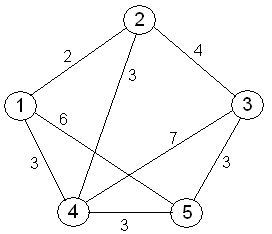
\includegraphics[scale=0.5]{imagens/tsp-sample.jpg}
	\end{center}
	\legend{Fonte: Google Images}
\end{figure}


O TSP pode ser representado por um grafo completo $G = (N, A)$, com $N$ sendo o conjunto de nós, também chamado cidades, e $A$ sendo o conjunto de arcos totalmente conectados aos nós. Cada arco $(i, j)$ pertencente $A$ é atribuído um valor $d_ij$ que representa a distância entre as cidades $i$ e $j$.

Tomando o exemplo da Figura \ref{fig:tsp-sample}, temos um grafo de cinco vértices em que cada aresta, associada a um vértice, possui um peso. Pensando em encontrar o percurso que passe em todos nós uma única vez, temos duas possíveis soluções ilustradas na Figura \ref{fig:tsp-exemplo}. É possível perceber que, ao somar o peso de todas as arestas do percurso, a rota ilustrada a esquerda possui menor tamanho se comparado a da direita. 

\begin{figure}[h]
	\caption{\label{fig:tsp-exemplo}Visualização de soluções em grafo.}
	\begin{center}
	    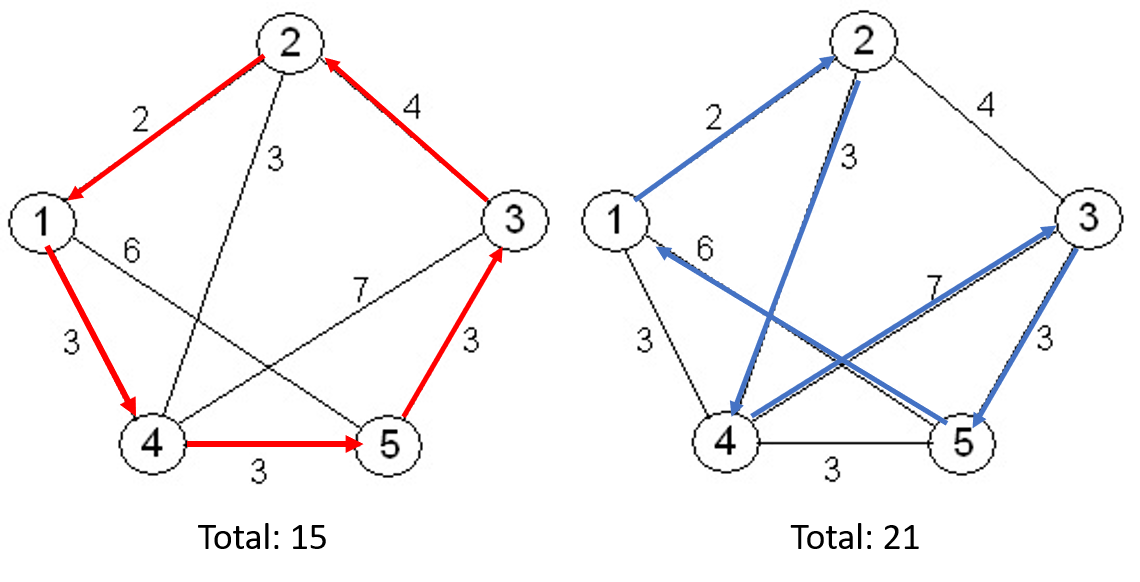
\includegraphics[scale=0.5]{imagens/grafos.png}
	\end{center}
	\legend{Fonte: O próprio autor}
\end{figure}

Logo, o TSP é um problema de encontrar um caminho fechado mais curto visitando cada um dos $n = |N|$ nós de $G$ exatamente uma vez. Para insâncias de TSP simétricos, as distâncias entre as cidades são independentes da direção transversal dos arcos, isto é, $D_ij = d_ji$ para cada par de nós. No TSP assimétrico pelo menos para um par de nós temos $d_ij \leq d_ji$.

% ---
\section{O Problema da Mochila (KP)}
\label{sec-kp}
% ---

O problema da mochila (KP) pode ser enunciado da seguinte forma (MARTELLO; TOTH, 1990) \cite{Martello:1990:KPA:98124}:

\textit{Um viajante levará consigo apenas uma mochila para sua viagem (Figura \ref{fig:kp-sample}). Sua mochila possui uma dada capacidade e deve ser preenchida com alguns objetos que lhe sejam úteis durante a viagem. Cada objeto possui um peso e um dado valor para o viajante e este possui apenas uma unidade de cada objeto a ser escolhido. Quais objetos devem ser levados pelo viajante em sua mochila de forma a maximizar o valor da mochila?}

\begin{figure}[h]
	\caption{\label{fig:kp-sample}Problema da mochila: Como maximizar o valor com um peso máximo?}
	\begin{center}
	    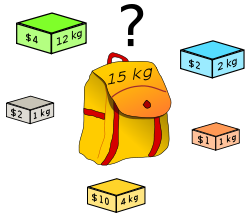
\includegraphics[scale=0.5]{imagens/kp-sample.png}
	\end{center}
	\legend{Fonte: Google Images}
\end{figure}

Seja $w_j$ o peso do $j$-ésimo objeto e $p_j$ seu valor. Se o objeto $x_j$ aparece na mochila, então  $x_j=1$ caso contrario $x_j=0$. Se denotarmos por $c$ a capacidade da mochila, e por $n$ a quantidade de objetos disponíveis para escolha e $F_(c)$ como o maior valor obtido para a mochila de capacidade $c$ usando os $n$ objetos, então o problema pode ser formulado algebricamente como a seguir:

\begin{equation} \label{eq:taco-ret} 
F_{(c)} = max\sum_{j=1}^{n} p_{j}x_{j} \quad (p_{j} > 0 )
\end{equation}

\begin{equation} \label{eq:taco-ret} 
sujeito \quad a\sum_{j=1}^{n} w_{j}x_{j} \leq c \quad (w_{j},c > 0 )
\end{equation}

onde: $x_j=0$ ou $x_{j}=1$.

Esta versão do problema é conhecida como problema da mochila binária (\textit{Binary KP} ou \textit{0-1KP}); Martello e Toth 1990 \cite{Martello:1990:KPA:98124}.

Se permitirmos a \(x_{j}\) assumir qualquer valor inteiro maior que zero então temos a forma mais genérica da versão unidimensional do problema da mochila. De acordo com a definição presente no trabalho de Martello e Toth 1990 \cite{Martello:1990:KPA:98124}, tal problema é conhecido como problema da mochila ilimitada (\textit{Unbounded Knapsack Problem} ou UKP).

Martello e Toth afirmam que, apesar do nome, o problema da mochila não é útil apenas na solução de problemas de empacotamento. Existem também aplicações na área da criptografia, engenharia naval, gerenciamento de projetos e finanças entre outras.

% ---
\section{Otimização e Problemas Multi-Objetivos}
\label{sec-multi}
% ---

É imprescindível o estudo de problemas multi-objetivo visto que a maior parte dos problemas do mundo real tendem a ser classificados desta forma. Augusutine (2002) \cite{augustine2002offline} explica que a complexidade dos problemas reais que surgem nas sociedades tecnológicas modernas é caracterizada pela existência de múltiplas perspectivas de análise, refletindo aspectos econômicos, sociais, políticos, físicos, de engenharia, administrativos, psicológicos, éticos, estéticos, etc.

Bastos-Filhos e Guimarães (2013) \cite{bastos2015multi} resumem o conceito de otimização como sendo “a busca por soluções para determinado problema (ou problemas) que o satisfaçam da melhor maneira possível”. Collette e Siarry (2013) \cite{collette2013multiobjective}, em seu livro “Multiobjective Optimization: Principles and Case Studies”, definem um problema de otimização como sendo a busca de um mínimo ou máximo (o ótimo) de uma função. O autor também descreve um caso específico de otimização chamado problema de otimização restrita. Este tipo ocorre quando problemas de otimização para os quais as variáveis da função a serem otimizadas são restritas para evoluir em uma área precisamente definida do espaço de pesquisa.

\begin{figure}[htb]
	\centering
	\caption{\label{fig:hotel-multi}Dilema de reserva de um quarto de hotel em função de dois objetivos: preço e conforto.} 
	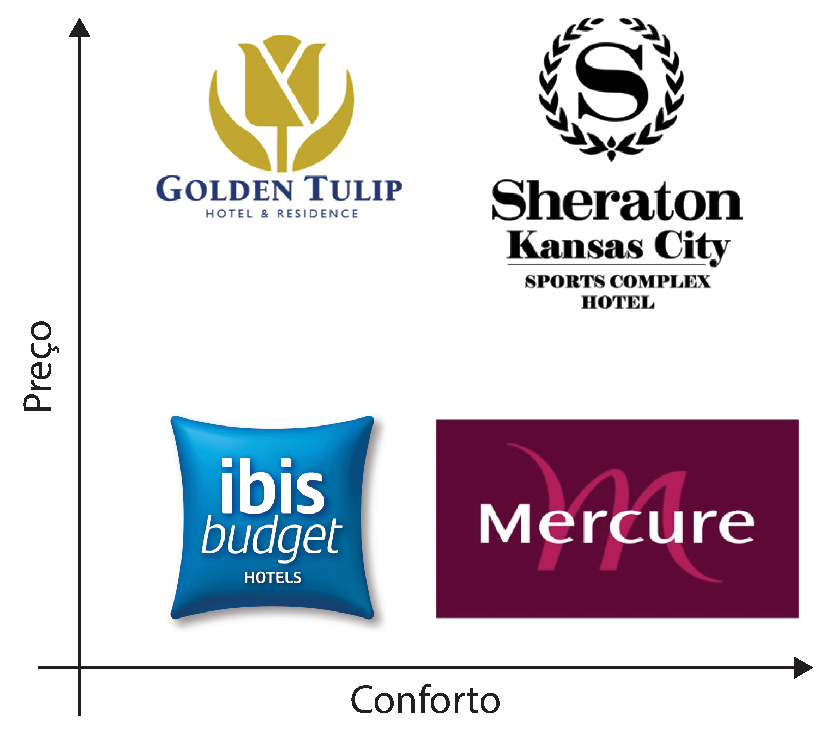
\includegraphics[width=0.5\textwidth]{imagens/hotel-multi.eps}
	\legend{Fonte: o próprio autor.}
\end{figure}

Branke et al. (2008) \cite{branke2008multiobjective} explicam que um problema de otimização mono objetivo envolve uma única função objetivo (ou função \textit{fitness}) e geralmente resulta em uma solução única, chamada de solução ótima. Por outro lado, uma tarefa de otimização multi-objetivo considera vários objetivos conflitantes simultaneamente. Nesse caso, geralmente não há solução ótima única, mas um conjunto de alternativas com diferentes compensações, chamadas de soluções ótimas de Pareto, ou soluções não dominadas.

A Figura \ref{fig:hotel-multi} apresenta um problema para a reserva de hotel, levando em consideração dois objetivos: preço e conforto. Se a pretensão for por um quarto com maior conforto, o preço será mais alto. Já, se pretende um quarto com menor preço, o conforto também será afetado, diminuindo-o.

